\documentclass{beamer}

\usepackage[frenchb]{babel}
\usepackage[T1]{fontenc}
\usepackage[utf8]{inputenc}
\usepackage{hyperref}

\usetheme{Warsaw}

\title{Diagramme de Voronoï et triangulation de Delaunay}
\author{Simon Mauras}
\institute{ENS Lyon}
\date{14 Janvier 2015}

\begin{document}

\begin{frame}
  \titlepage
\end{frame}

\begin{frame}
  \frametitle{Sommaire}
  \tableofcontents
\end{frame}

\section{Présentation du problème}

\subsection{Voronoï et problèmes de Clustering}

\begin{frame}
  \begin{block}{Clustering}
    \begin{itemize}
      \item Analyser des données de manière automatique
      \item Voronoï : Calcul de l'ensemble des plus proches voisins dans un espace metrique.
    \end{itemize}
  \end{block}

  \begin{block}{Cas particulier : en dimension 2}
    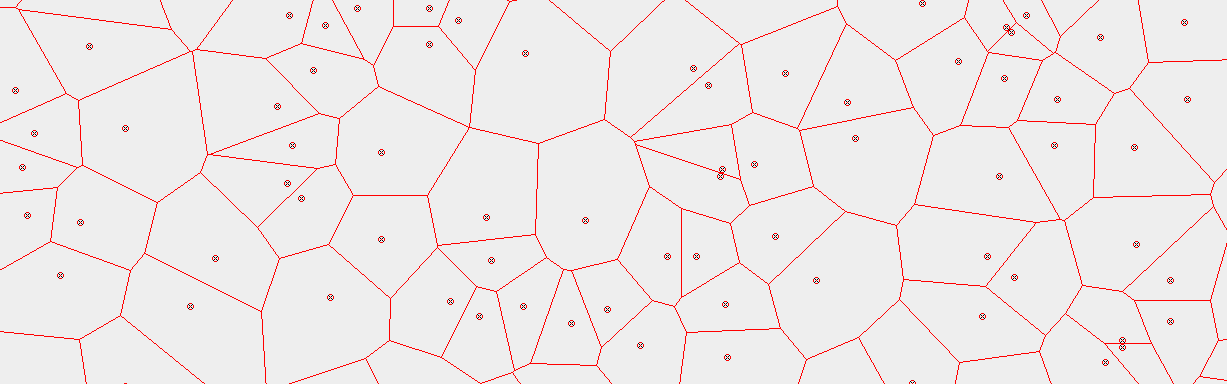
\includegraphics[width=\textwidth]{voronoi.png}
  \end{block}
\end{frame}
  
\subsection{Graphe dual et triangulation de Delaunay}

\begin{frame}
  \begin{block}{Graphe dual et triangulation de Delaunay}
    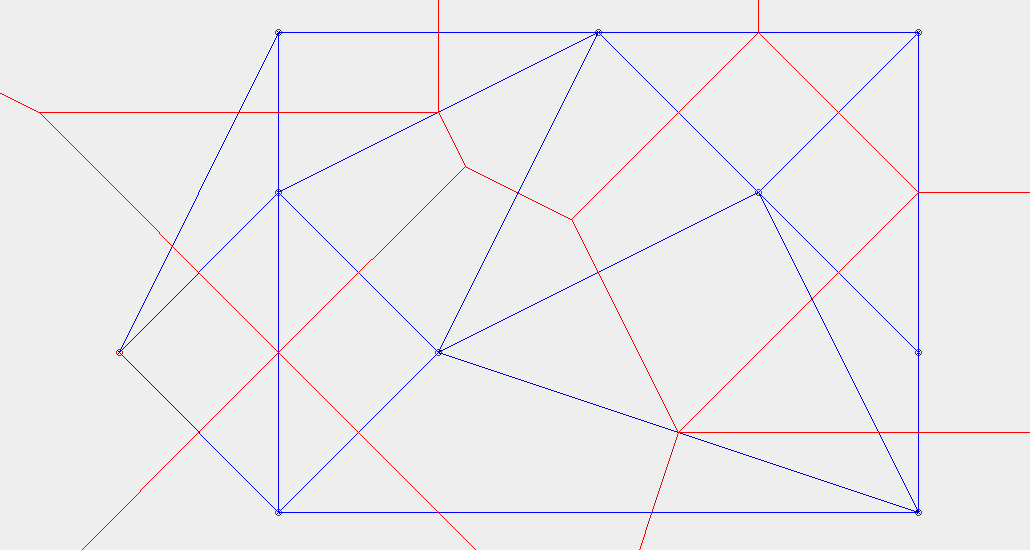
\includegraphics[width=\textwidth]{dual.png}
  \end{block}
\end{frame}

\section{Historique des solutions apportées}

\begin{frame}
  \begin{block}{Rappel chronologique des algorithmes proposés}
    \begin{description}
      \item[1975] Shamos, Hoey : Diviser pour régner (Voronoï)\\
        $\mathcal O(n \log n)$ dans le pire des cas.
      \item[1978] Green, Sibson : Incrémental (Voronoï)\\
        $\mathcal O(n \log n)$ en moyenne, $\mathcal O(n^2)$ dans le pire des cas
      \item[1980] \textbf{Lee, Schachter (triangulation de Delaunay)}
      \item[1987] Fortune : Balayage (Voronoï)\\
        $\mathcal O(n \log n)$ dans le pire des cas.
    \end{description}
  \end{block}
\end{frame}

\begin{frame}
  \begin{block}{Algorithmes de Lee et Schachter}
    ``Two Algorithms for Constructing a Delaunay Triangulation''\\
    \small{\textit{International Journal of Computer and Information Sciences}, Jun 1980}
    \begin{itemize}
      \item \textbf{Diviser pour régner} : $\mathcal O(n \log n)$ dans le pire des cas.
      \item Itératif : $\mathcal O(n \log n)$ en moyenne, $\mathcal O(n^2)$ dans le pire des cas.
    \end{itemize}
  \end{block}
\end{frame}

\section{Algorithme de Lee et Schachter}

\begin{frame}
  \begin{block}{Algorithme}
    \begin{overlayarea}{\textwidth}{6cm}
      \only<1>{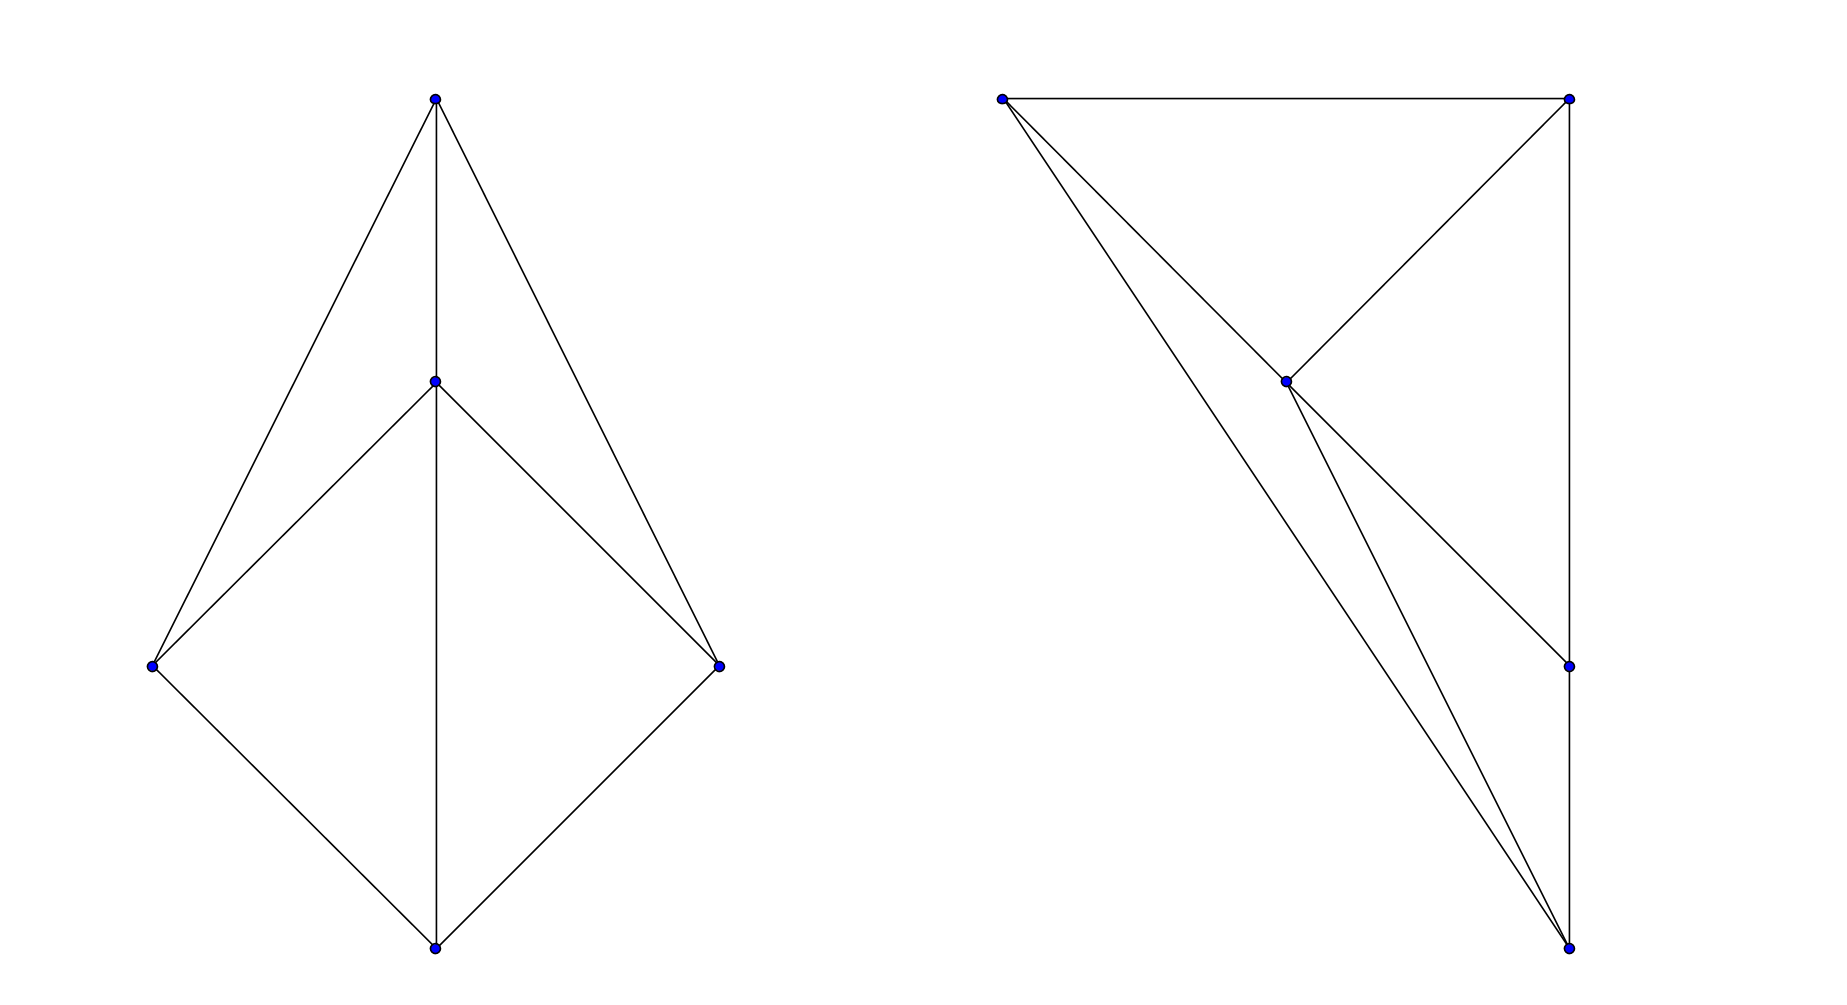
\includegraphics[width=\textwidth]{1.png}}
      \only<2>{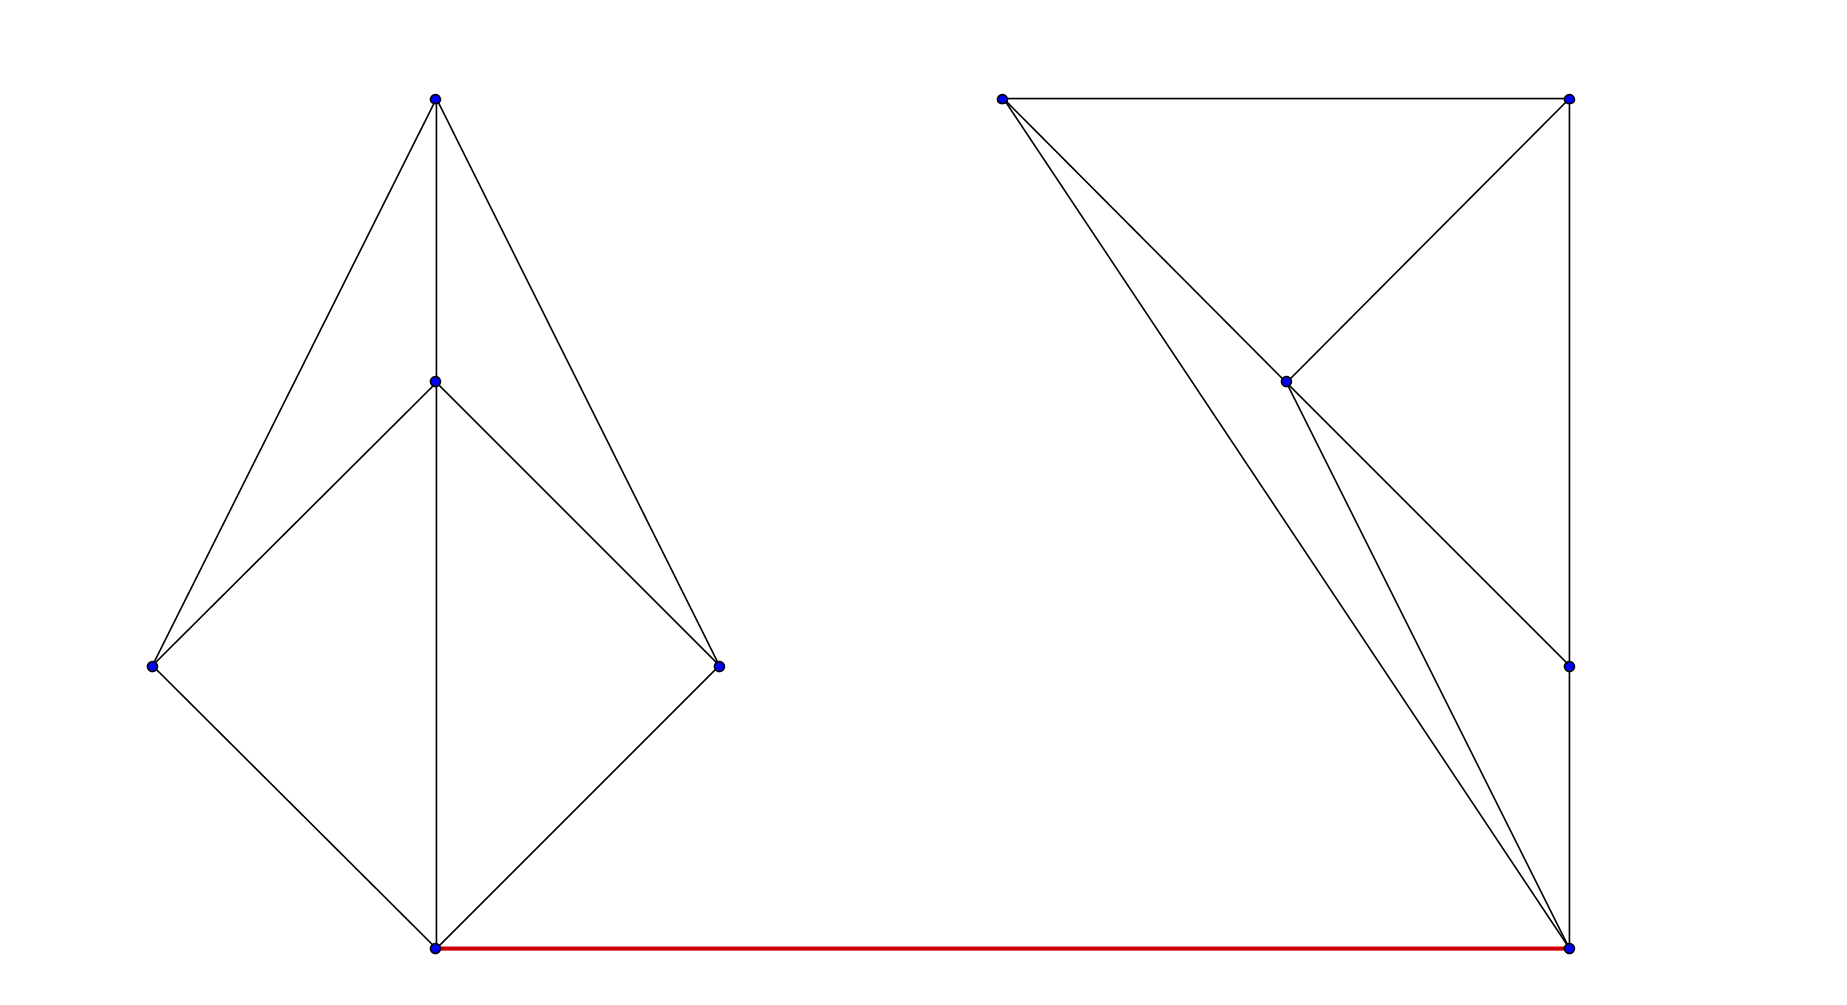
\includegraphics[width=\textwidth]{2.png}}
      \only<3>{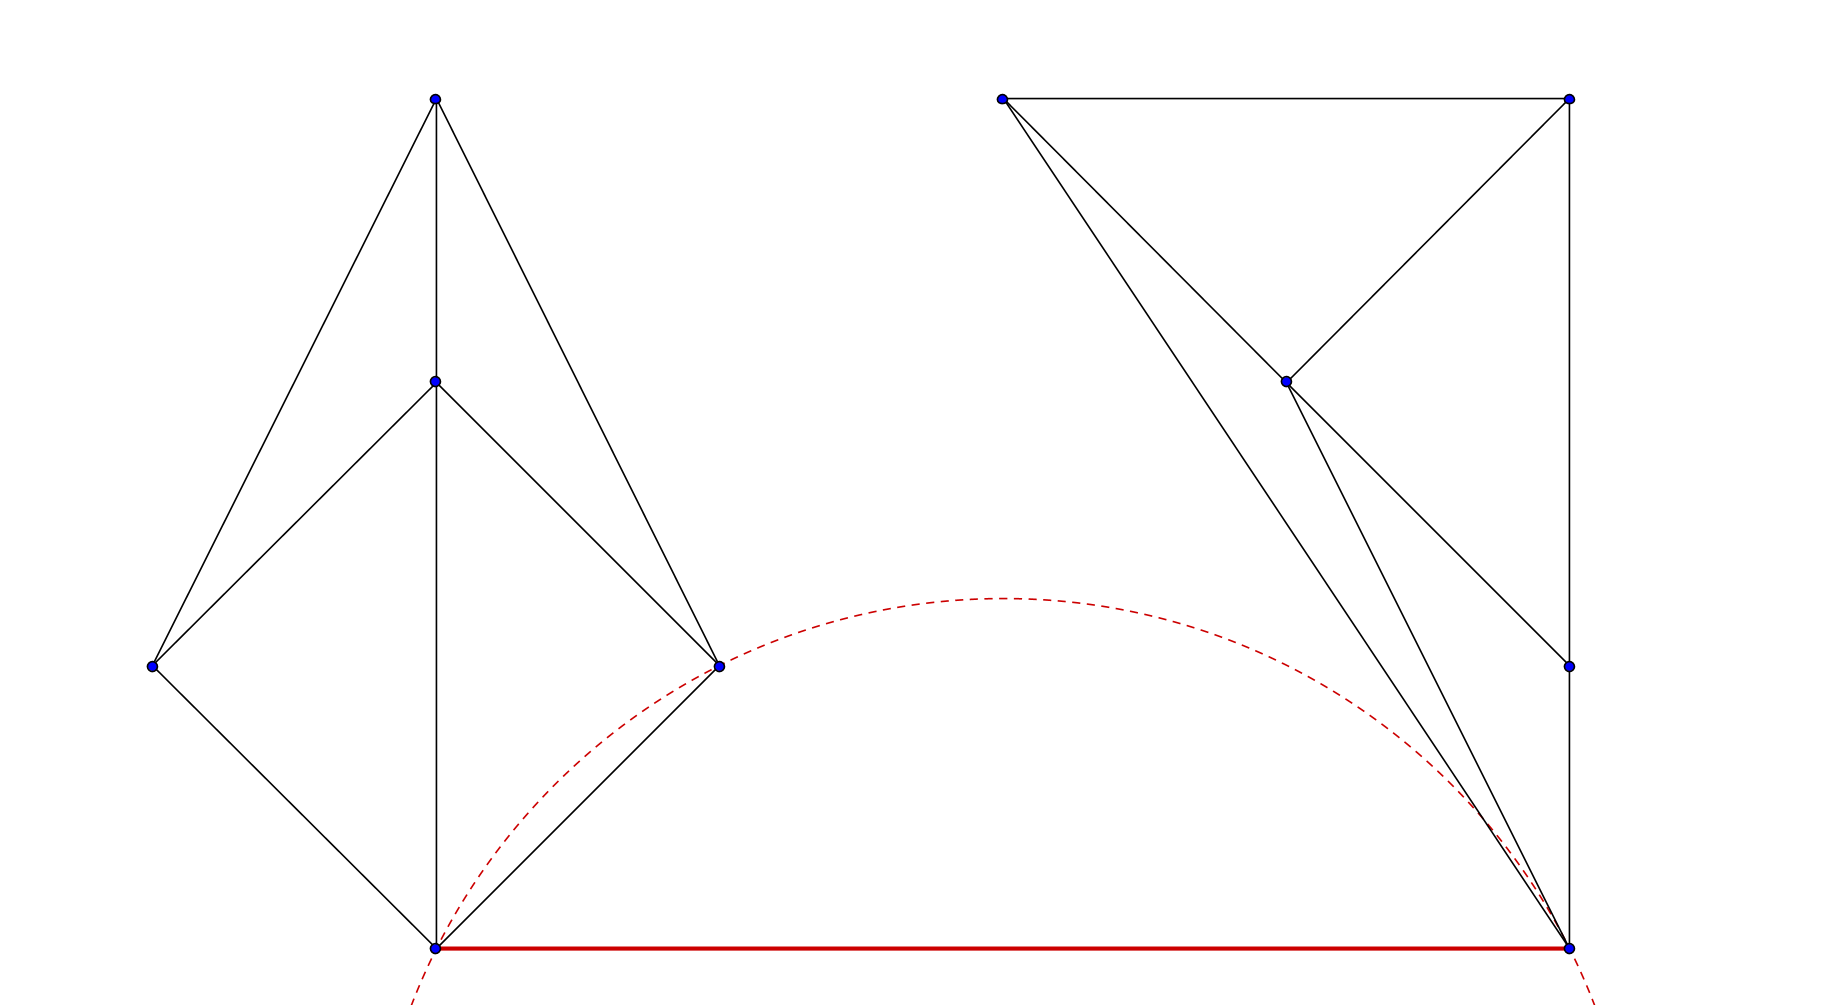
\includegraphics[width=\textwidth]{3.png}}
      \only<4>{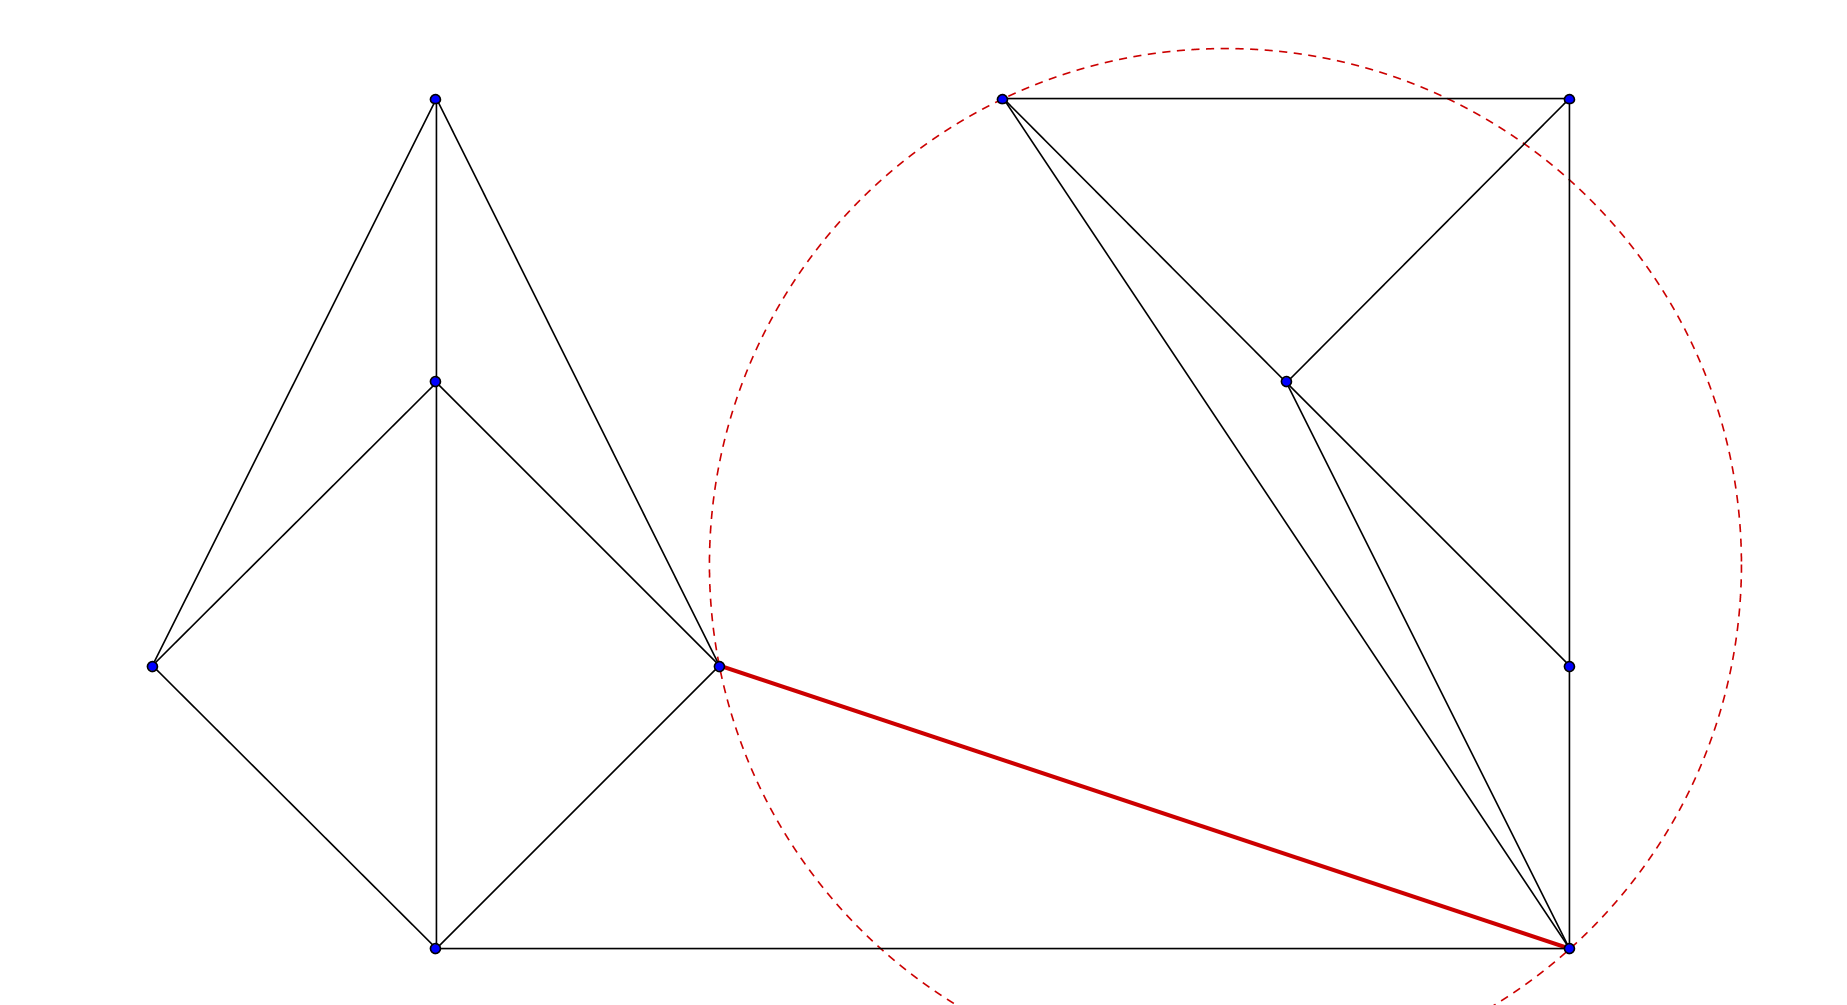
\includegraphics[width=\textwidth]{4.png}}
      \only<5>{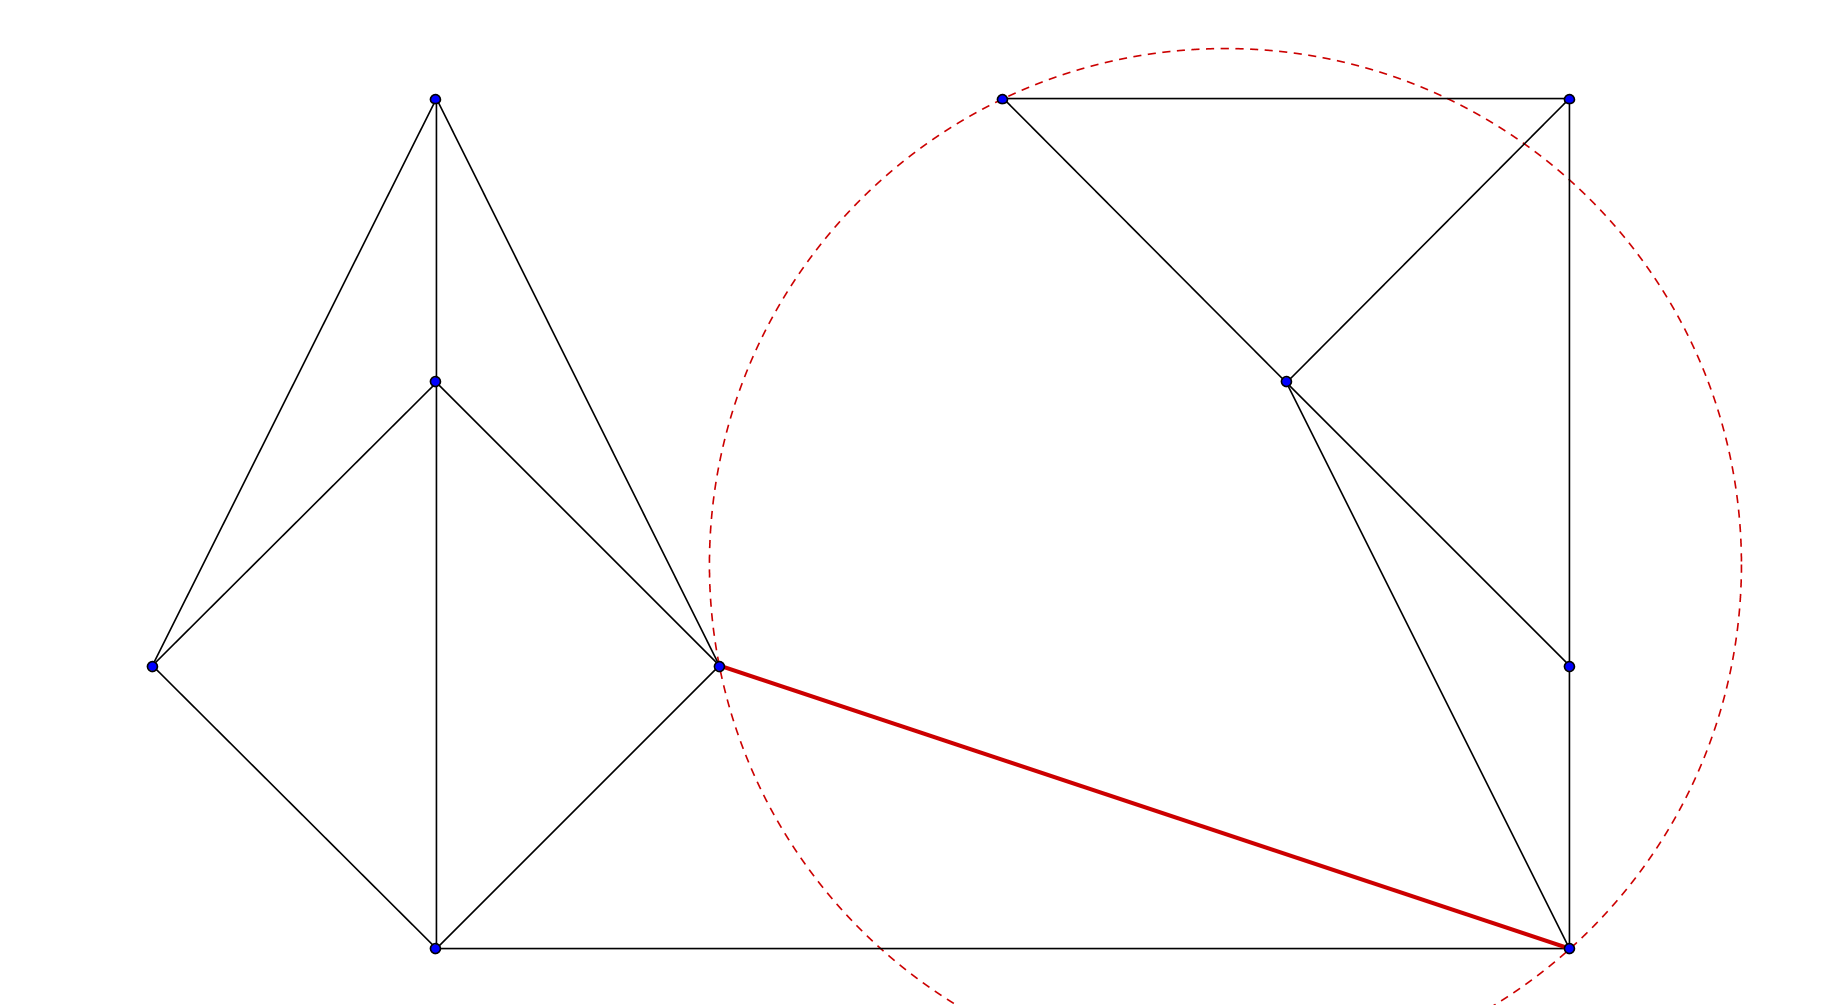
\includegraphics[width=\textwidth]{5.png}}
      \only<6>{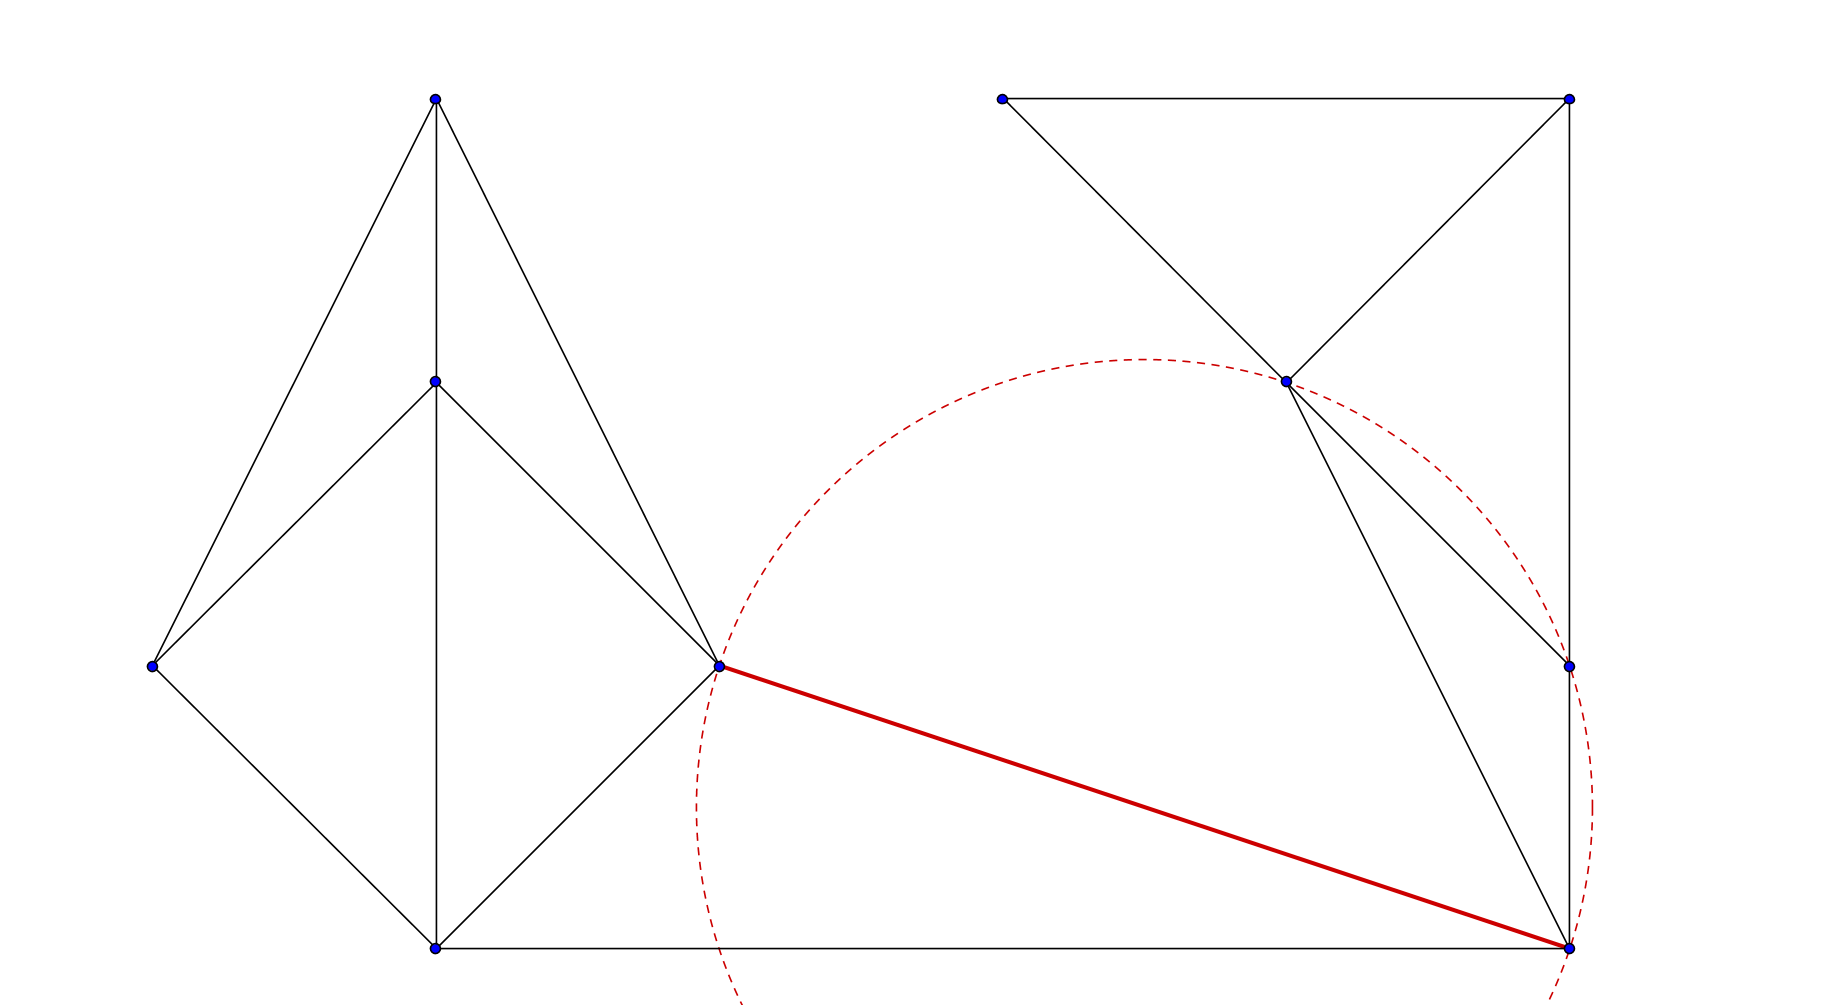
\includegraphics[width=\textwidth]{6.png}}
      \only<7>{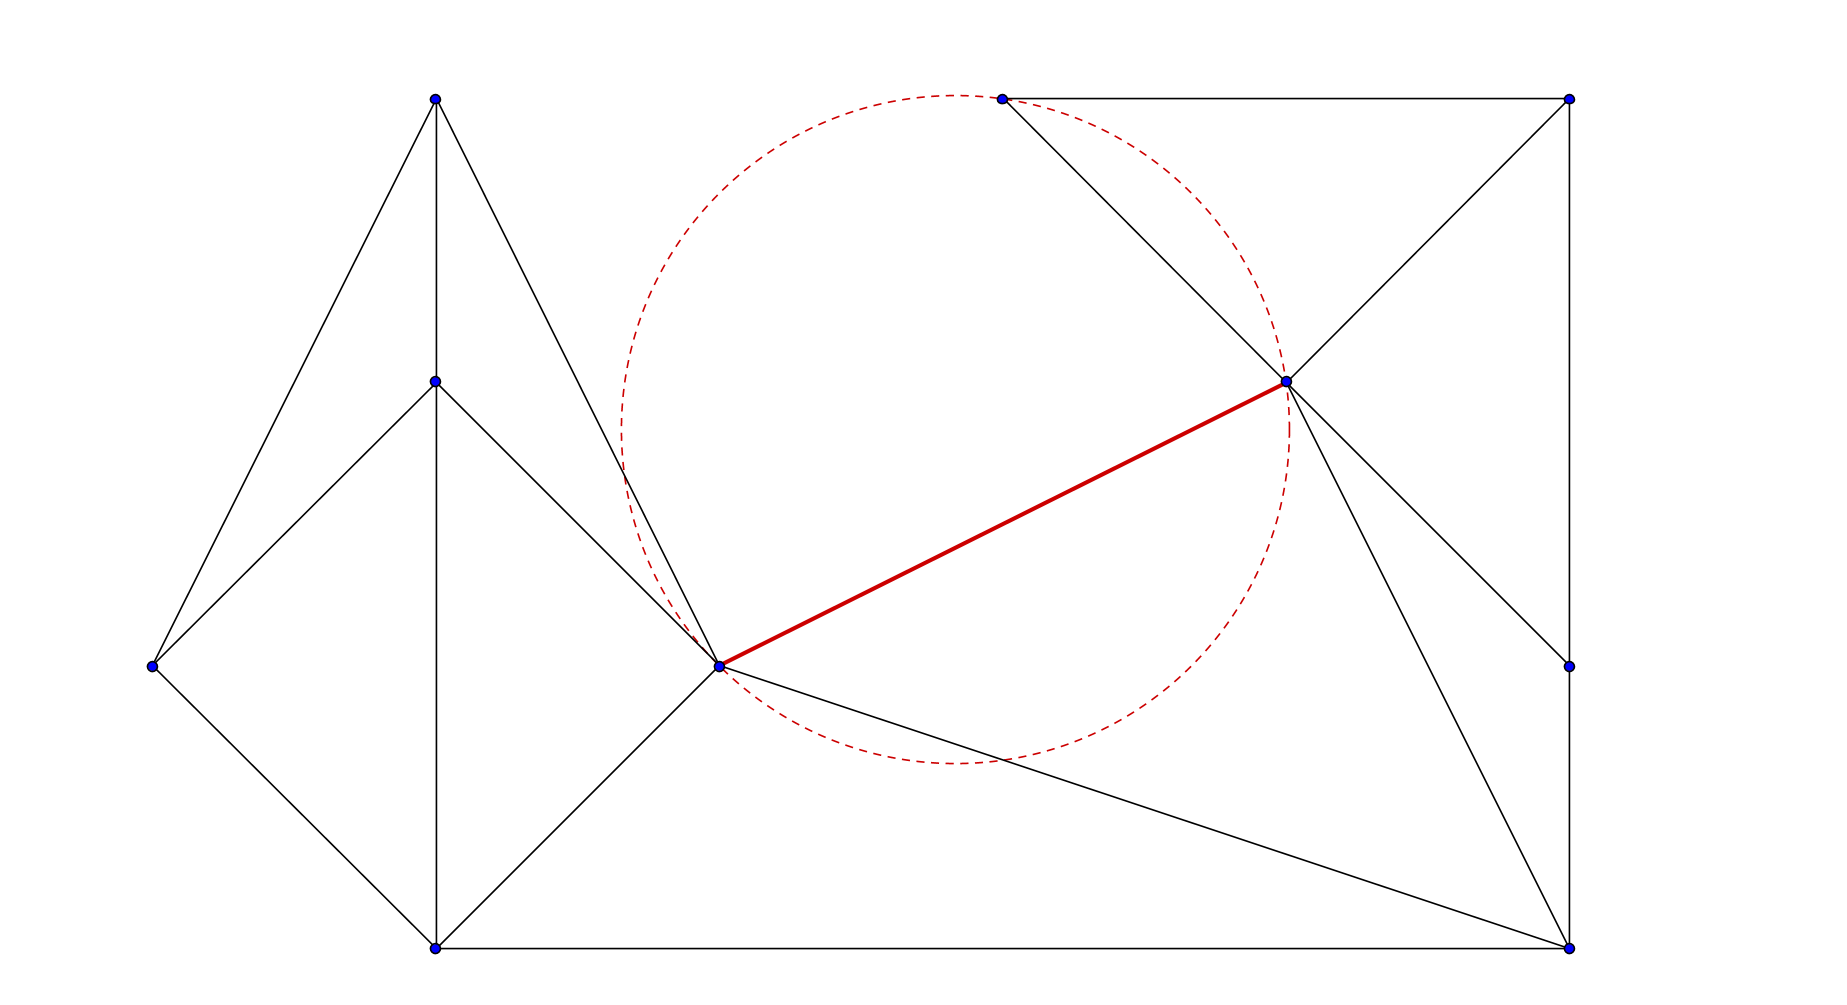
\includegraphics[width=\textwidth]{7.png}}
      \only<8>{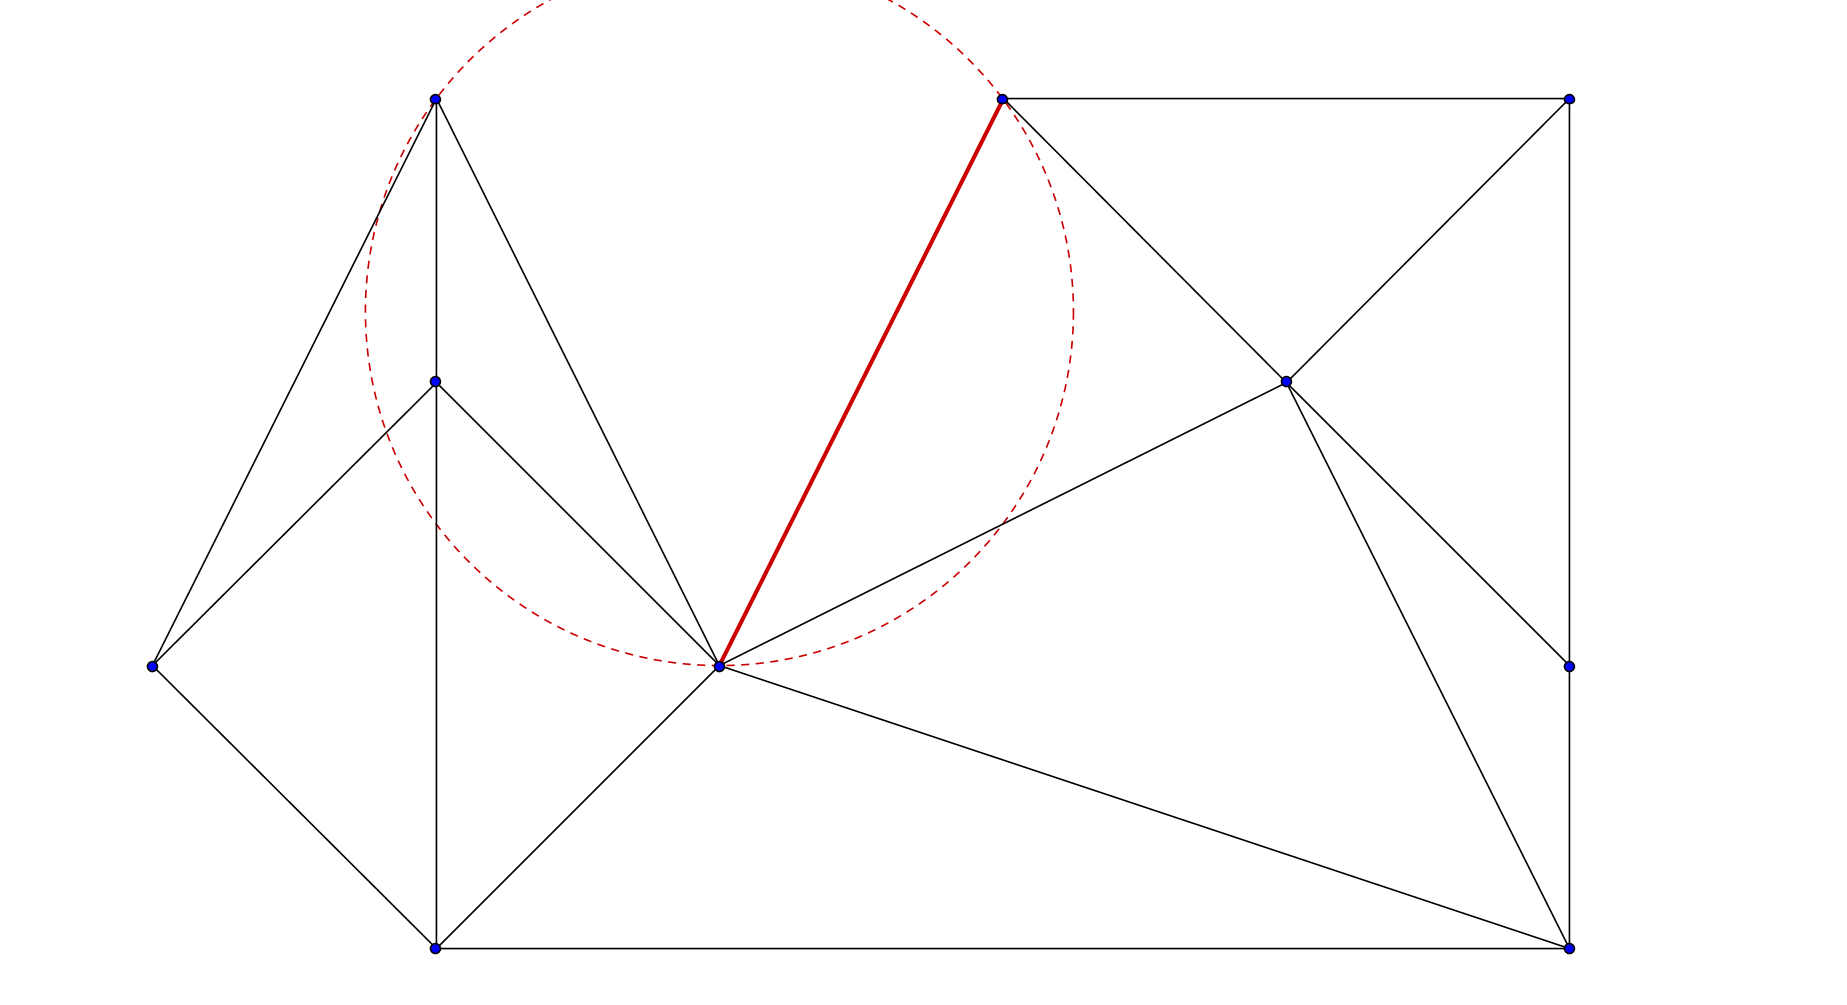
\includegraphics[width=\textwidth]{8.png}}
      \only<9>{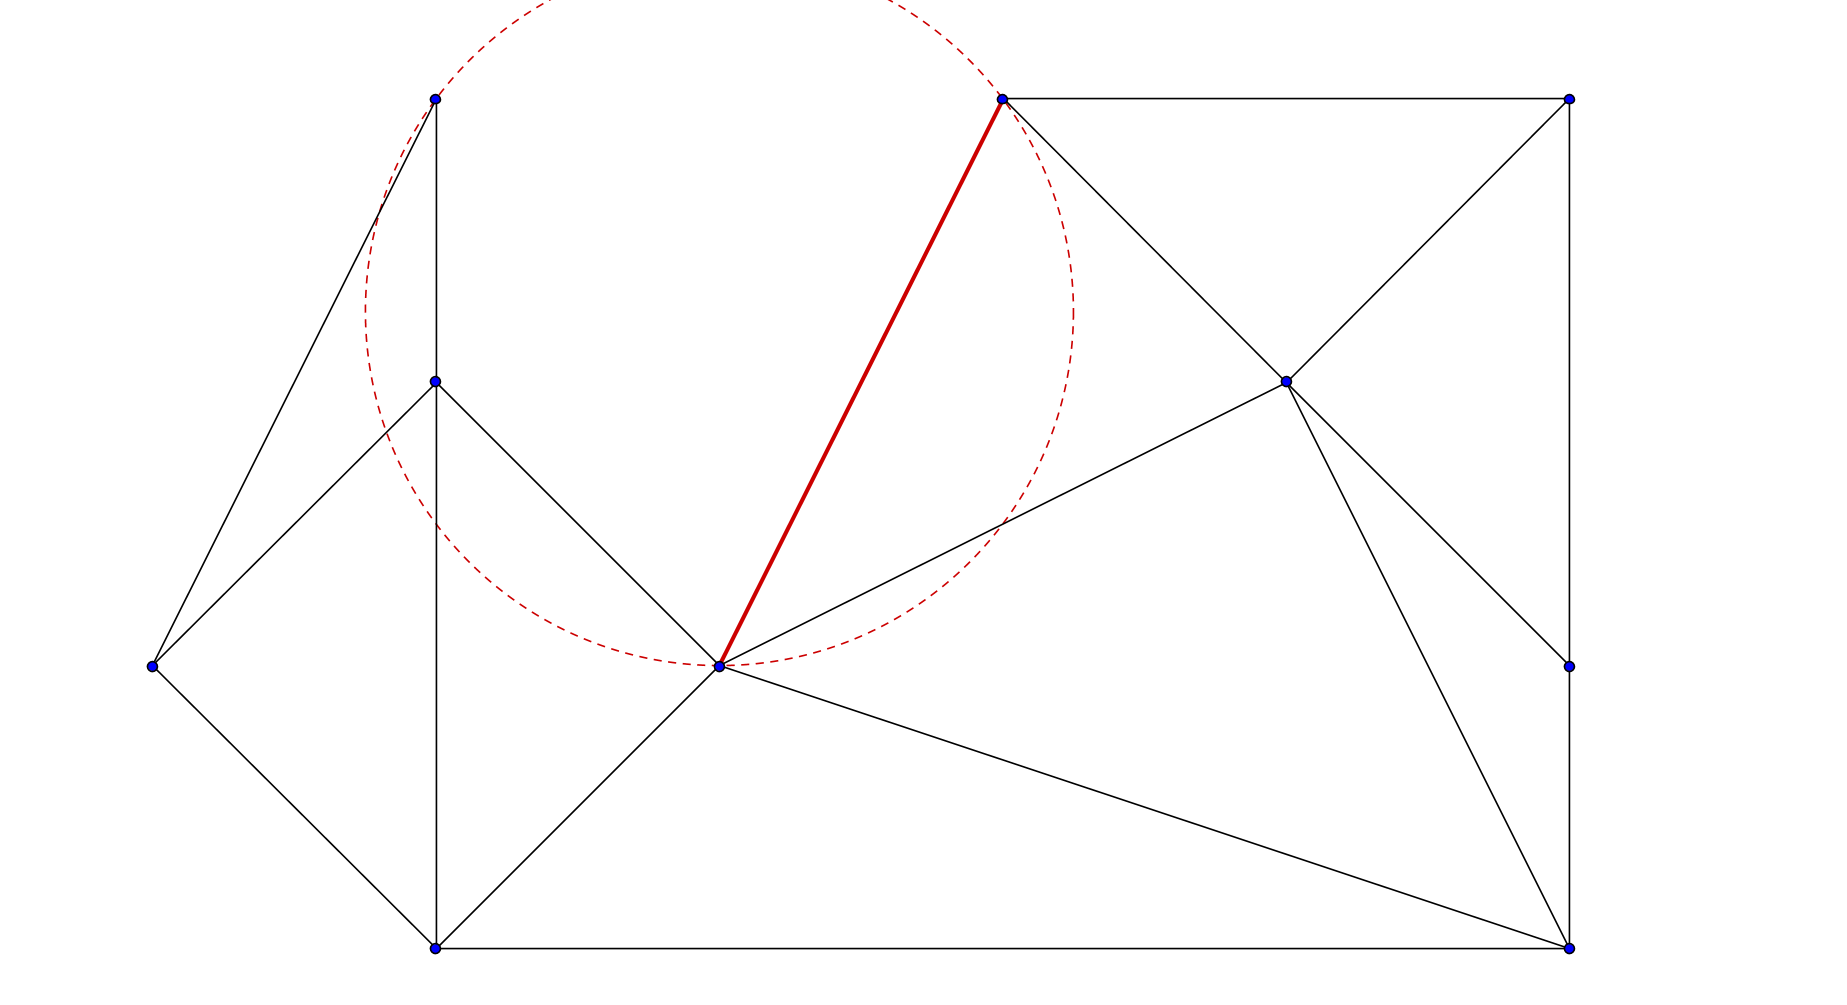
\includegraphics[width=\textwidth]{9.png}}
      \only<10>{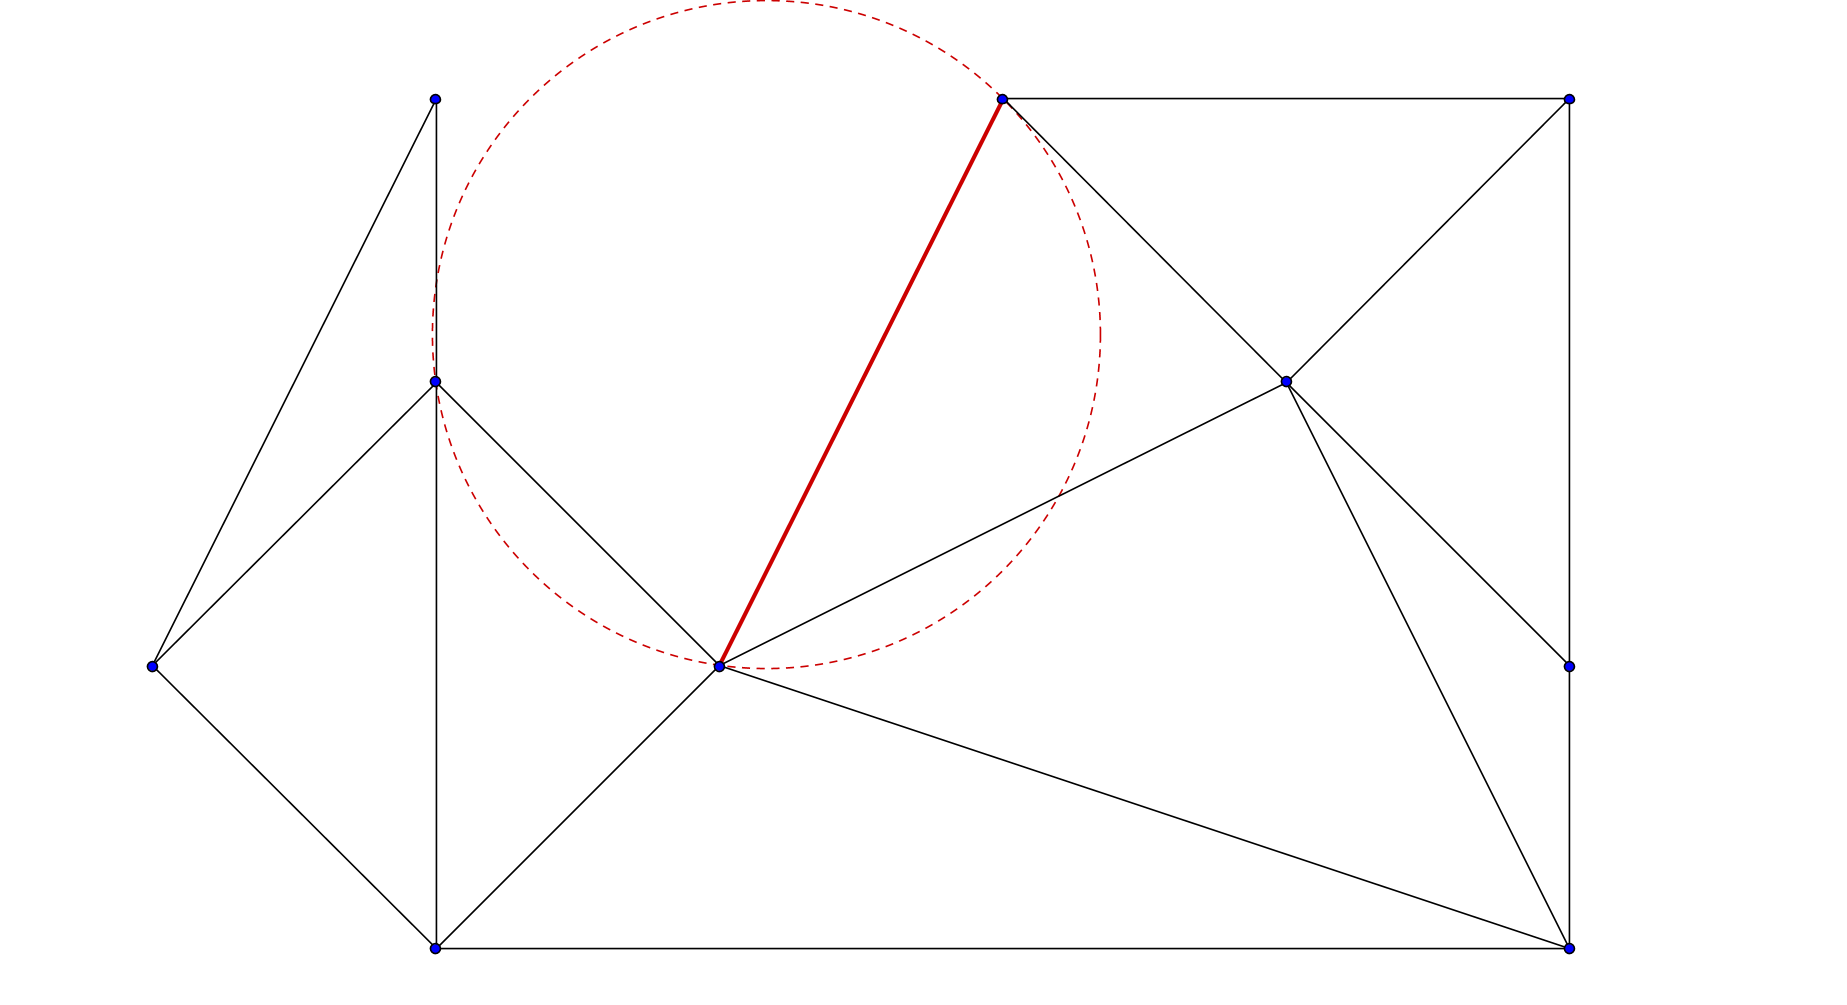
\includegraphics[width=\textwidth]{10.png}}
      \only<11>{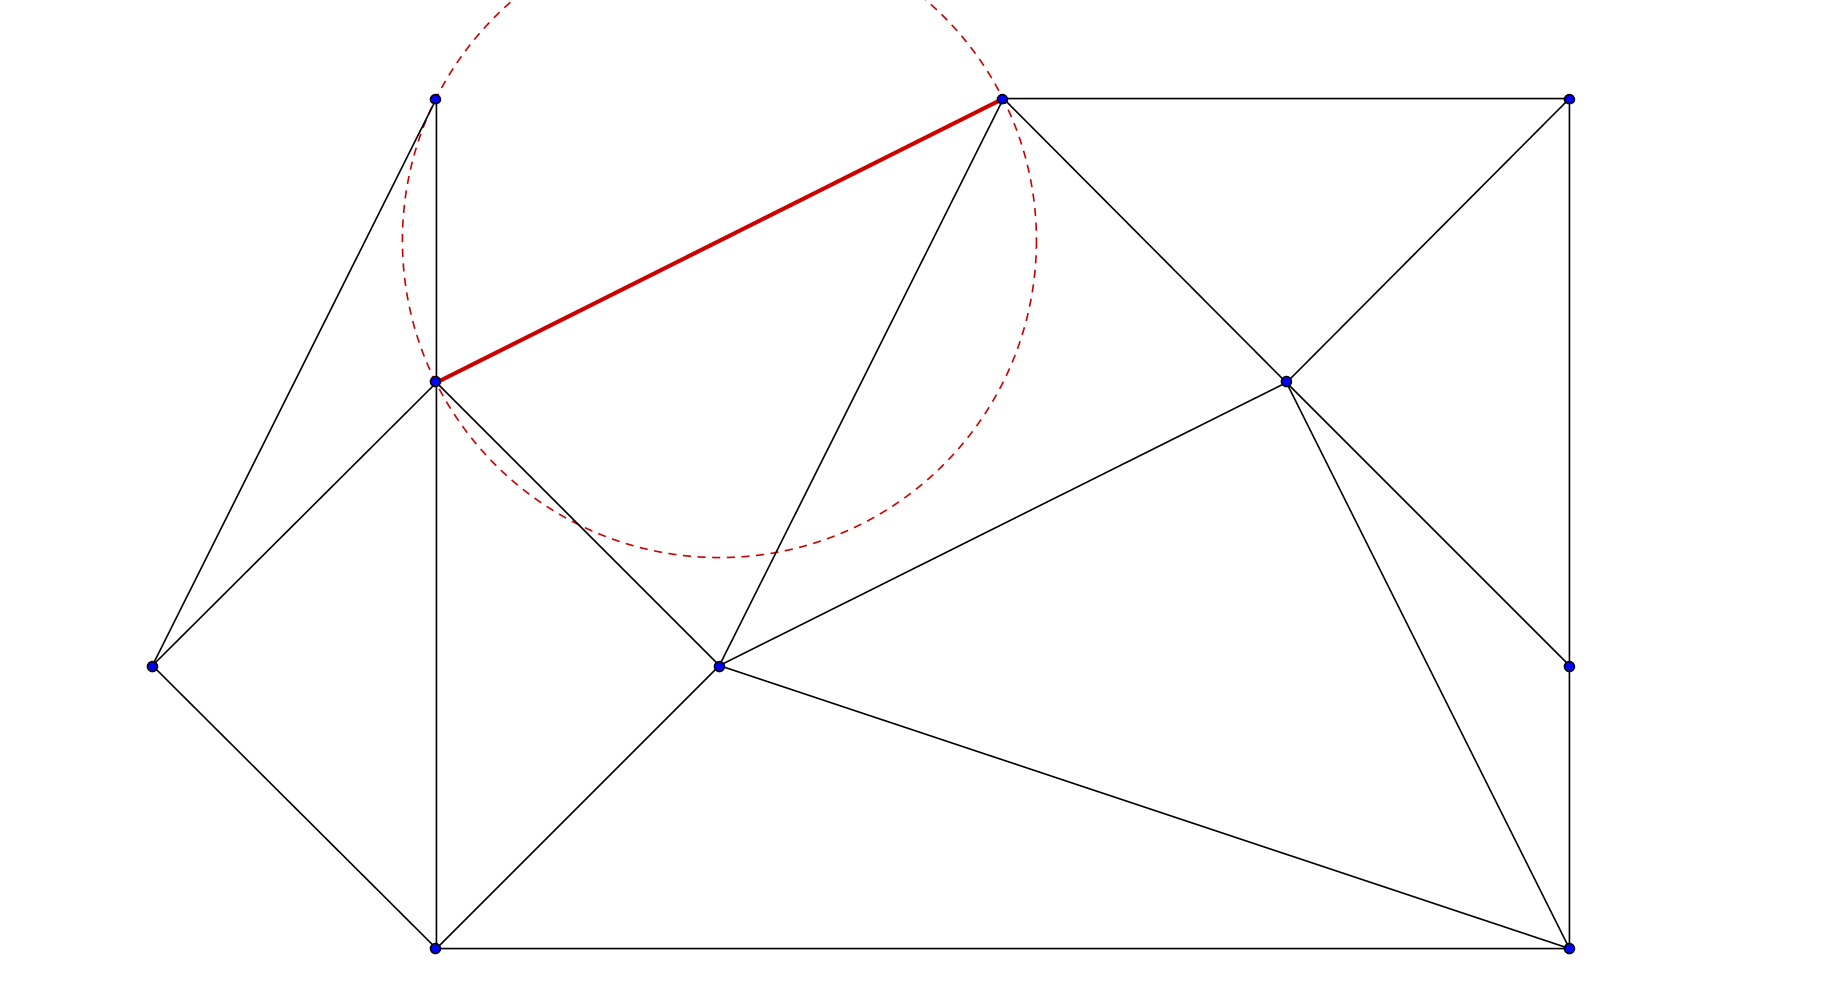
\includegraphics[width=\textwidth]{11.png}}
      \only<12>{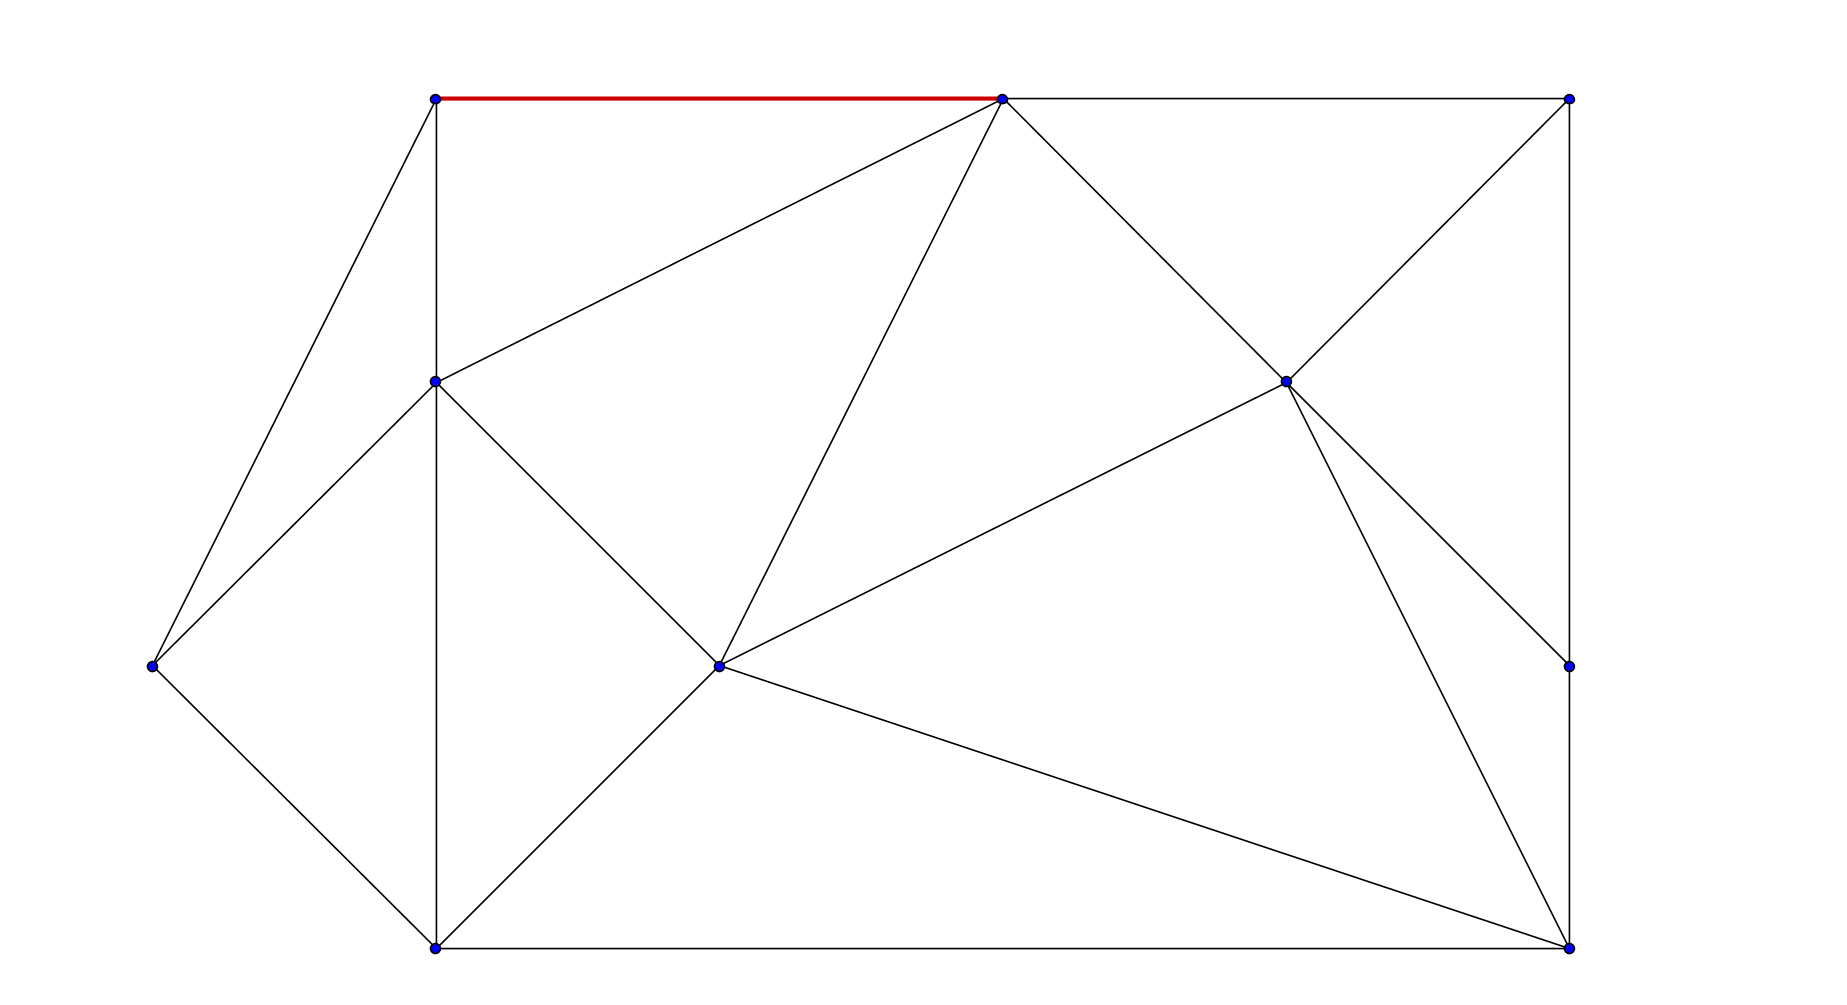
\includegraphics[width=\textwidth]{12.png}}
      \only<13>{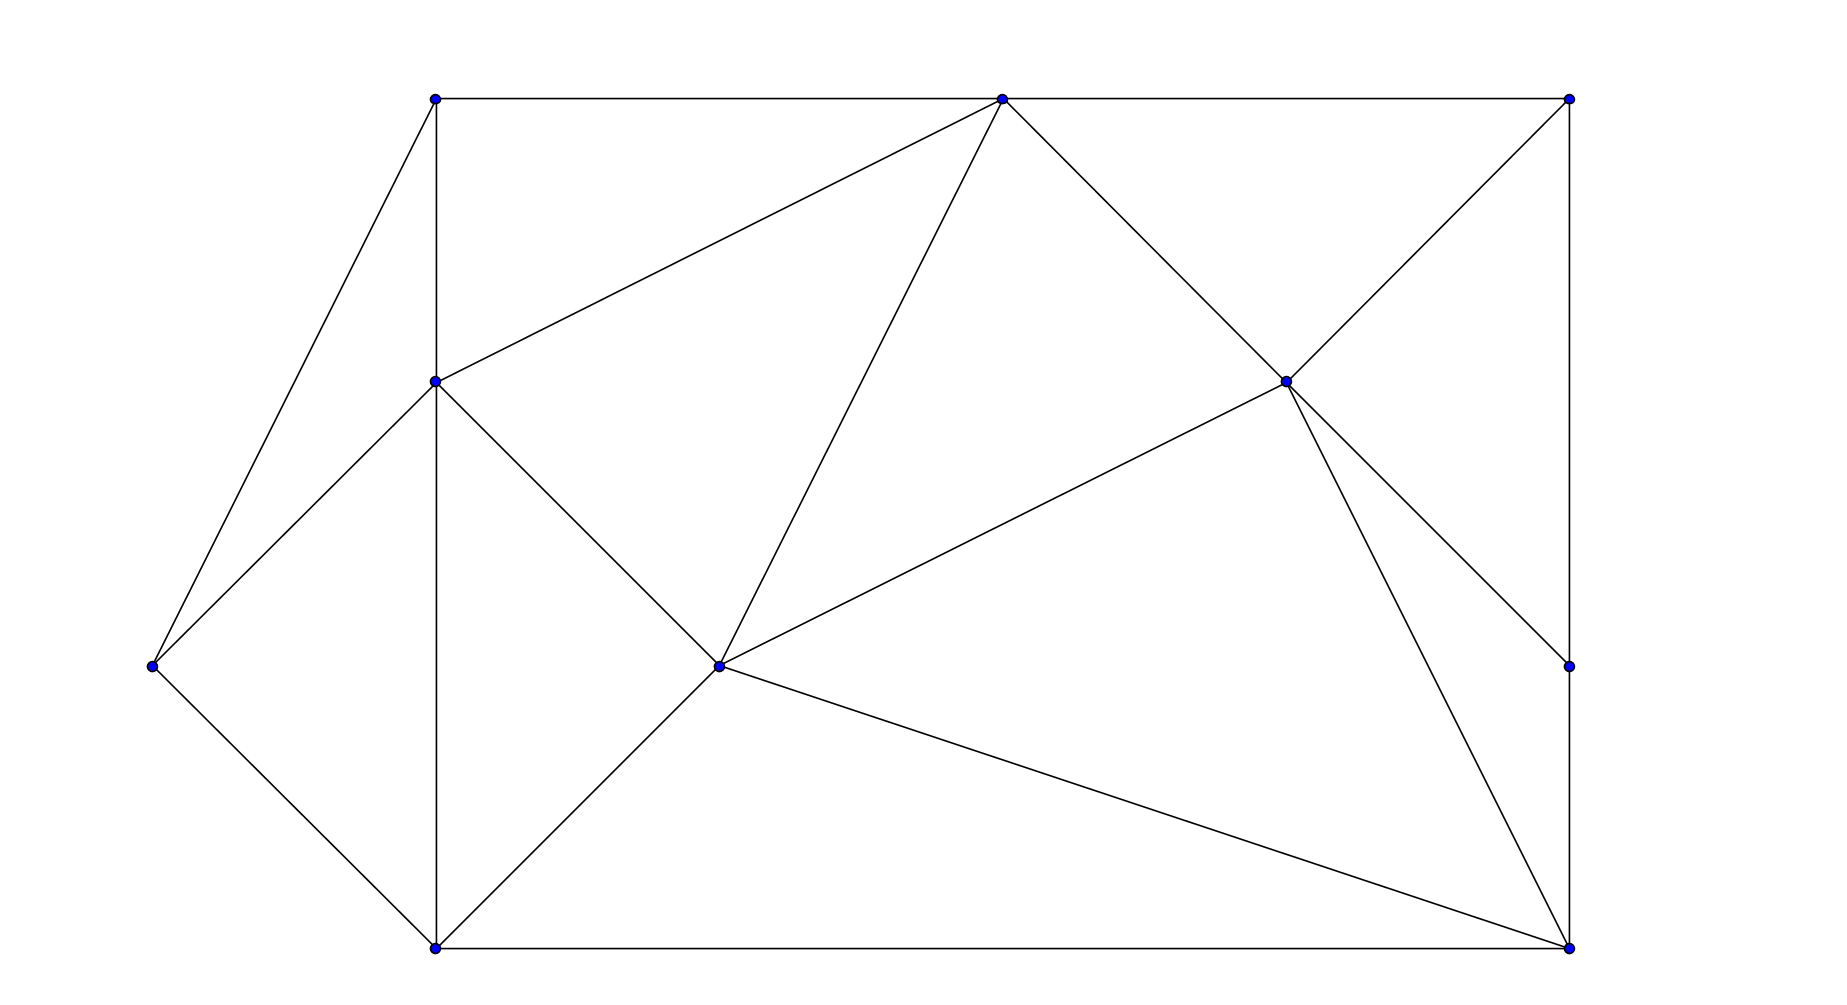
\includegraphics[width=\textwidth]{13.png}}
    \end{overlayarea}
  \end{block}
\end{frame}

\begin{frame}
  \frametitle{Références}
  \begin{itemize}
  \item D.T. Lee, B.J. Schachter, ``Two Algorithms for Constructing a Delaunay Triangulation'', \textit{International Journal of Computer and Information Sciences}, Jun 1980
  \item S. Peterson, ``Computing constrained Delaunay triangulations'', \href{http://www.geom.uiuc.edu/~samuelp/del_project.html}{[en ligne, consulté en janvier 2015]}
  \end{itemize}
\end{frame}

\end{document}
